 % -*- root: ../../twm.tex -*-

\section{Obtaining Data}

\begin{frame}
    \frametitle{Obtaining}
    \begin{itemize}
        \item Ready to use data sets
        \begin{itemize}
            \item Gold standard corpora
            \item Classification: Reuters Newswire, Twenty Newsgroups, Youtube Spam, ...
            \item Sentiment: reviews from Amazon, TripAdvisor, Rotten Tomatoes, ...
        \end{itemize}
        \item APIs
        \begin{itemize}
            \item Twitter, New York Times, Guardian
            \item Only in real time?
        \end{itemize}
        \item Crawling / Scraping
        \begin{itemize}
            \item Data for (almost) any domain of interest
            \item Legal? Terms of Service, robots.txt
        \end{itemize}
    \end{itemize}
\end{frame}


\begin{frame}
    \frametitle{Gold Standard Corpora}
    \textcolor{iseblue}{Wissler et al. (2014)}
    \begin{itemize}
        \item Standard collections for training and evaluation of algorithms
        \item Manual annotations and more structure thain plain text
    \begin{itemize}
        \item Syntactical information, lexical knowledge, semantic associations
        \item E.g. entities, grammatical structures
    \end{itemize}
    \item Multiple experts view the data independently
    \begin{itemize}
        \item Inter-annotator agreement
        \item Creation is time-consuming and expensive
    \end{itemize}
    \item Example: Penn Treebank
    \begin{itemize}
        \item 4.5 million English words, GSC for syntactical tagging
    \end{itemize}
    \end{itemize}
\end{frame}

\subsection{Legality of Web Scraping}
\begin{frame}
    \frametitle{Legality of Web Scraping}

\begin{itemize}
    \item It is public anyway / Google does it
    \begin{itemize}
    \item Added value by search engines
    \item What about log in systems, paywalls, ...?
    \end{itemize}
\end{itemize}

\begin{itemize}
    \item Highly context specific
    \begin{itemize}
    \item Commerical v non-commercial
    \item Internal v third party use
    \end{itemize}
\end{itemize}

\begin{itemize}
    \item Technicalities
    \begin{itemize}
    \item Humans don't access thousands of pages, bandwidth usage
    \item Denial-of-service (DoS) attack
    \end{itemize}
\end{itemize}

\end{frame}


\begin{frame}
    \frametitle{European Union}
    \begin{itemize}
        \item \textcolor{iseblue}{Ryanair Ltd v PR Aviation BV (2015)}
        \begin{itemize}
            \item PR Aviation: price comparison of flights
            \item Copyright and database right infringement?
            \item ToS prohibited data extraction for commercial purposes
        \end{itemize}
            \end{itemize}
        \begin{itemize}
        \item Decision by Court of Justice of the European Union
        \begin{itemize}
            \item No infringement of intellectual property, no creative input
            \item ToS still apply, liability in terms of breach of contract
        \end{itemize}
    \end{itemize}
    \vspace{5pt}
        \begin{itemize}
        \item In contrast \textcolor{iseblue}{NLA v Meltwater (2013)}
        \begin{itemize}
            \item Scraping of news headlines and links to articles
            \item Intellectual property is infringed because of creative input
        \end{itemize}
    \end{itemize}
\end{frame}

\begin{frame}
    \frametitle{United States}
Pro \\
\begin{itemize}
    \item Web data is public, should be accessible
    \item First Amendment protects information gathering
    \item Unfair market power of Facebook, Google, LinkedIn, ...
\end{itemize}
\vspace{8pt}
Contra \\
\begin{itemize}
    \item Copyright infringement
    \item Breach of contract
    \item Violation of the Computer Fraud and Abuse Act (CFAA), 1986 \\
        $\quad \;$forbids unauthorized access to some computers
    \item Trespass to chattels
\end{itemize}
\end{frame}

\begin{frame}
    \frametitle{LinkedIn v hiQ and vice versa}
{
\center
\textit{
\large
If you exclude someone from sites like LinkedIn, Facebook and Twitter, you are excluding them from the modern version of the town square. }
} \\
\vspace{-10pt}
\begin{flushright}
Laurence Tribe, Harvard law professor
\end{flushright}
\vspace{10pt}
\begin{itemize}
    \item hiQ - startup predicting who is when quitting their job
    \item LinkedIn: CFAA violation, hiQ: blocked
    \item LinkedIn ordered to give access to public profiles
\end{itemize}
\end{frame}

\begin{frame}
    \frametitle{Academia is save, right?}
    \setlength\tabcolsep{1.pt}
      \begin{tabular}{cl}
      \setlength\tabcolsep{1.5pt}
         \begin{tabular}{c}
           
\includegraphics[scale=0.15]{img/figures/aaron_swartz.jpg}
           \end{tabular}
           & \begin{tabular}{l}
            \small
             \parbox{0.7\linewidth}{%  change the parbox width as appropiate
             \textbf{Aaron Swartz} 
             \begin{itemize}
    \item Harvard research fellow
    \item Automatic download of articles from JSTOR
    \item Download via laptop in a closet at MIT
    \item No civil law suit by MIT and JSTOR
    \item Federal charges: wire fraud, CFAA violations
    \item Possible penalty of \$1 million and 35 years in prison
\end{itemize}
\vspace{10pt}
Unclear outcome, suicide on January 11, 2013
    }
         \end{tabular}  \\
\end{tabular}   
\end{frame}

\begin{frame}
    \frametitle{Good Manners and Ethics}
\begin{itemize}
    \item Data as a product
    \item Cost of bandwidth
    \item Rapid requests slow services for real humans
    \item robots.txt
\end{itemize}
\end{frame}

\begin{frame}
    \frametitle{Google's robots.txt}
\begin{figure}[htb]
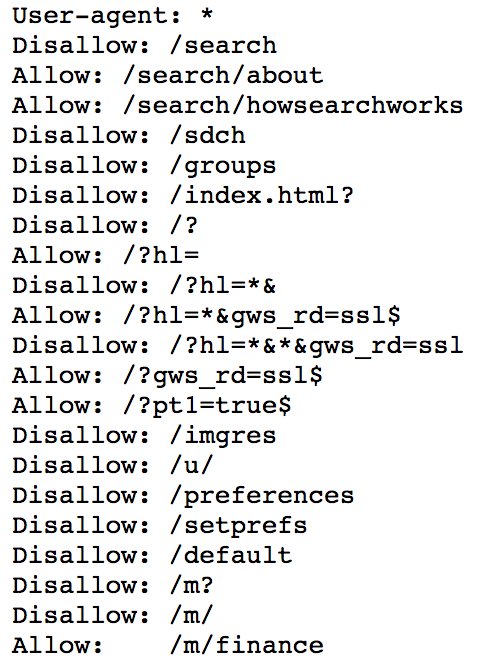
\includegraphics[scale=0.27,left]{img/figures/google_robots}
\end{figure}
\end{frame}

\begin{frame}
    \frametitle{Ethical Scraping for Academia}
\begin{itemize}
    \item Technical
    \begin{itemize}
    \item Use API if provided
    \item Appear as a bot, not as a human
    \item Provide user agent string with contact data
    \item Decreased rate of requests
    \end{itemize}
    \end{itemize}
    \vspace{5pt}
    \begin{itemize}
    \item Usage
    \begin{itemize}
    \item Strictly non-commercial
    \item Restrict further access to academia
    \end{itemize}
\end{itemize}
    \vspace{5pt}
    \begin{itemize}
    \item Ask for permission, not for forgiveness!
    \end{itemize}
\end{frame}

\begin{frame}
    \frametitle{Scraping and Crawling}

\end{frame}

\begin{frame}
    \frametitle{Scraping How To}

\end{frame}

\begin{frame}
    \frametitle{Beer Advocate}

\end{frame}

\begin{frame}
    \frametitle{Individual Review}
    \vspace{-25pt}
    \begin{figure}[htb]
        \begin{center}
            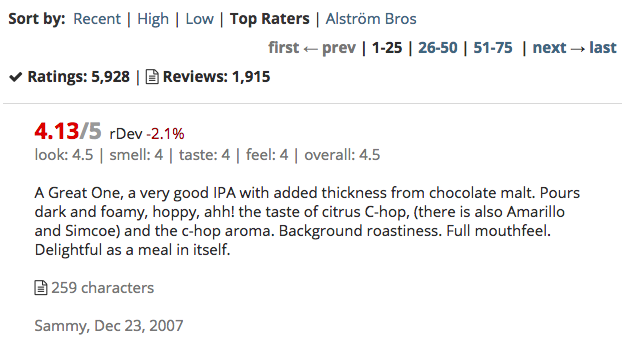
\includegraphics[scale=0.5]{img/figures/rating}
        \end{center}

\end{figure}
\vspace{-20pt}
\begin{flushright}
\textcolor{iseblue}{\href{https://www.beeradvocate.com/beer/profile/147/38470/?view=beer&sort=topr&start=0}{Source}}
\end{flushright}
\end{frame}

\begin{frame}
    \frametitle{xPath Inspector}
    \vspace{-25pt}
    \begin{figure}[htb]
        \begin{center}
            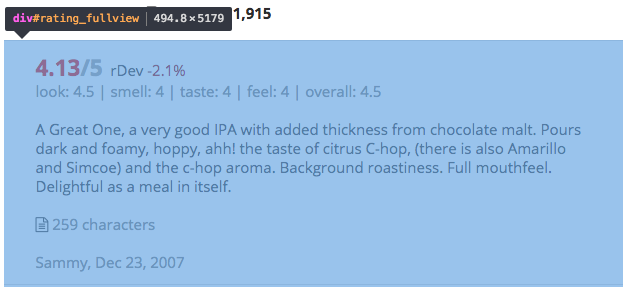
\includegraphics[scale=0.5]{img/figures/xpath}
        \end{center}

\end{figure}
\vspace{-20pt}
%\verb | //*[@id="rating_fullview_content_2"]|

\end{frame}


\frame[plain]{
    \center \LARGE \bf
    \color{isegreen} Example: \href{http://localhost:8888/live_examples/scraper.ipynb}{Scraper}
}